\documentclass[journal]{IEEEtran}

% \usepackage{cite}
\usepackage[sort&compress, numbers]{natbib}
\usepackage{graphicx} % to use graph, tables, etc
\usepackage{float} % to fix the image location
\usepackage{amsmath}
\usepackage{url}
\usepackage{amsmath}
\usepackage{fixltx2e}
\usepackage{stfloats}
\usepackage{gensymb} % easier chemical and physics symbol unit declaration
\usepackage{tabularx,ragged2e,booktabs,caption}
\newcolumntype{C}{>{\Centering\arraybackslash}X} % 
\hyphenation{op-tical net-works semi-conduc-tor}

\usepackage[font=footnotesize]{caption}
% \usepackage{subcaption}
\begin{document}

\title{Fully-Conformable Skin Sensors for Sports\\Fatigue Detection}

\author{\textbf{Nathaniel Wihardjo$^{1,2}$, 
        S. William Sunanto$^{1,3}$,
        A. Kenny Oktavius$^{1,4}$, \\
        Olivia Winata$^{1,5}$, 
        Jin Li$^{1,6}$, 
        Ping Gao$^{1,7}$} \\
        {\small 
            \textsuperscript{1}Department of Chemical and Biomolecular Engineering Hong Kong University of Science and Technology \\
            \textsuperscript{2}nwihardjo@ust.hk
            \textsuperscript{3}swsunanto@ust.hk
            \textsuperscript{4}akoktavius@ust.hk
            \textsuperscript{5}owinata@ust.hk
            \textsuperscript{6}jlicm@ust.hk
            \textsuperscript{7}kepgao@.ust.hk}}% <-this % stops a space

% The report headers
\markboth{HKUST CBE Final Year Project 2019}%do not delete next lines
{Shell \MakeLowercase{\textit{et al.}}: Bare Demo of IEEEtran.cls for IEEE Journals}

% make the title area
\maketitle

\markboth{HKUST CBE Final Year Project 2019}%do not delete next lines
{Shell \MakeLowercase{\textit{et al.}}: Bare Demo of IEEEtran.cls for IEEE Journals}

% make the title area
\maketitle

\begin{abstract}
Over these years, wearable biosensors development has been rising as a promising technology which revolutionizes the conventional health monitoring methods. It is capable of giving precaution warnings when there is health problem detected and thus, informing the users to halt their exercises. In professional sports environment, it is crucial for an athlete to know their physical limit and adjust their workout methods accordingly. However, the current existing method is still too bulky which makes it not breathable and difficult to conform with the skin. We had successfully fabricated sweat sensors based on the Ultra-High-Molecular-Weight Polyethylene (UHMWPE) membrane with a thickness range about 100 nanometers. As a result, it conforms perfectly to the skin without the need of any adhesives. From testing its capability to collect sweat as biomarker and analyzing the collected sweat composition through Raman and Energy Dispersive Spectroscopy (EDS), we have found the presence of stress hormone called cortisol which is an accurate indicator of fatigue level. The developed cortisol-sensing device using the first-ever self-standing, nano-level UHMWPE membrane opens a lot of research areas in the healthcare industry as well as providing more favourable technology to monitor athletes’ physical performance based on consultations with Hong Kong Sports Institute (HKSI).
\end{abstract}

\begin{IEEEkeywords}
Biomarker, Sweat, Fatigue, Cortisol, Ultra-High-Molecular-Weight-Polyethylene 
\end{IEEEkeywords}

\section{iIntroduction}
\IEEEPARstart{T}{he} development of athlete’s physical performance has been immensely fast, shown by various records that were broken in every summer Olympic; it is undeniable how sports are evolving by time. Cynthia Bir, the  lead  scientist  for  ESPN’s  “Sport  Science”  show,  explained  how  science  has improved athlete’s abilities and enabled them to reach points that were unthinkable decades ago~\cite{SkinSystems}. Biometric feedback is one of the methods used by the experts in optimizing athlete’s performance~\cite{Biofeedback}; it provides metrics which enable coaches to tailor trainings in order to help athletes pass a plateau. Sweat is not just merely one form of human perspiration, but it also acts as performance safety metrics for athletes. In professional athlete trainings, coaches often push athletes into the “red zone” in order to return stronger after certain adaptation period. The excitement of heightened performance brings the subsequent problem. Driven by high-ambition, both athlete and coach are keep pushing without any certain boundaries which results in a very vulnerable physical condition such as overtraining phenomenon which significantly lowered athletes’ performance for extended period of time, or in extreme cases, can lead to metabolic imbalances and chronic diseases of blood vessels, heart and others~\cite{OvertrainReviewDirections, ReviewOvertraining, ImmuneOvertraining}. Hence, it is very crucial for athletes to know their physical limit and adjust their workout methods accordingly.

This particular research area has been rapidly intensified all around the world. Stanford research group had developed a device which measures fatigue level from sweat~\cite{Parlak_membraneElectro}. However, their device is still too bulky and thus, not able to perfectly conform without the use of any adhesives as well as non-breathable. Herein, this project aims to develop a flexible, adhesive and stretchable nanolayer sweat sensing device to monitor athletes’ fatigue level both during vigorous exercise and non-workout condition through stress hormone called cortisol. This project is built on top of the developed first ever self-standing membrane based on UHMWPE which have the thickness down to 100 nanometers. 

Lee Wai-Sze, Hong-Kong’s best cyclist who has had tremendous achievements this year; contributed 2 gold medals in both Asian Games 2018 and UCI Track Cycling World Championship 2019. HKSI has been a prominent pillar behind all those medals achieved, providing a comprehensive training system which comprises of professional coaches, sports science and medicine. Their current method for detecting  fatigue  level  is  by measuring cortisol through blood plasma instead of sweat. The problem lies when the tests are performed in regular basis. According to Frankie Su from HKSI Sports Nutrition Monitoring Center, the invasive usage of finger prick has been proven not giving any convenience to majority of athletes. 

In addition, another issue brought up by HKSI were the time efficiency and accessibility. After collecting the blood samples, it took around 1 hour to analyze the composition and get the results. A more crucial case is when athletes are having practices or competition abroad, the test could not be performed at all since the blood-analysis machine cannot be carried easily. 

Herein, this project aims to develop conformable, non-invasive and stretchable nanolayer device to monitor athlete’s fatigue level both during vigorous exercise and non-workout environment through a stress hormone known as cortisol. The application itself is designed to be used for professional athletes as well as general use of non-athletes.

This paper will first further discuss the importance of cortisol in terms of sports fatigue measurement as well as the mechanism behind perspiration and human skin. Then in Chapter 3, device fabrication procedure and its installation to the skin will be reviewed along with thorough explanation of the experimentation and analysis method performed. Finally, Chapter 4 will discuss more into the novelty of the product, economic analysis, and some of the limitations and future works of this project.

\section{Literature Review}
\subsection{Skin Structure}

As the project mainly interacts with skin and the human perspiration, it is essential to discuss the mechanism and properties of both in advance. Skin consists of different layers, that each has its own unique function and characteristic. Epidermis is located on the most outer part, contains a lot of dead skin cells~\cite{PhysHumanPersp}. Epidermis is responsible for distributing melanin pigment to give color to the skin, skin’s adaptive immune responses, and receptors for touch response. On the inner side of epidermis, there are dermis layer that essentially is supporting matrix which are linked to its remarkable capacity for retaining water. There are two types of protein fibers in dermis that supports skin’s tensile strength as well as its elasticity and resilience~\cite{PhysHumanPersp}. Dermis is where the sweat glands located (Fig.~\ref{fig:skin}). 

\begin{figure}[H]
\centering
\includegraphics[width=0.35\textwidth]{images/skin.jpg}
\caption{Skin structure consisting of different layers}\label{fig:skin}
\end{figure}

The key role of skin is to provide a mechanical barrier against the external environment as well as thermoregulation. Vasodilation or vasoconstriction of the blood vessels under the skin helps regulate heat loss with eccrine sweat glands that can produce 2-4 litre of sweat per hour during moderate exercises, or up to 10-14 litre of sweat per day ~\cite{TemperatureRegulation, BodyFluid, Thermoregulatory}. This is the sweat that the proposed membrane collects and analyzes. The eccrine gland is responsible for thermoregulatory sweating in humans and hence, distributed over nearly the entire body surface. Its structure consists of a bulbous secretory coil which is located in the lower dermis, and the duct extends through the dermis and opens directly onto the skin surface.

\subsection{Perspiration}
 Human perspiration can be categorized into two: insensible perspiration and active sweating~\cite{PhysHumanPersp}. Insensible perspiration involves water loss from respiratory passages, skin and gaseous exchanges in the lungs. The evaporation from skin is supplied from water coming from blood in which depends on several environmental factors like ambient temperature and humidity. On the other hand, active sweating is induced by heat, muscular exercise, mental stimuli and carbon dioxide~\cite{PhysHumanPersp}. Thermal sweating holds an important role in maintaining body’s temperature which involves the whole-body surface, whereas emotional sweating often appears only on the palms and soles. 

The chemistry of perspiration lies on the mechanism of sweat excretion. On the sweat gland, intracellular Ca$^{2+}$ concentration increases which leads to the increase of the K$^+$ and Cl$^-$ permeability. As a result, isotonic precursor fluid from secretory cells are triggered and released~\cite{PhysHumanPersp}. As the fluid travels up the duct toward the surface of the skin, sodium and chloride are reabsorbed and causes the resulted sweat in the surface hypotonic relative to plasma. During a rigorous exercise, the rate of sweat production increases, ion reabsorption mechanisms can be overwhelmed since the quantity of sweat secreted into the duct is very large, resulting in a higher ion loss. 

Sweat produced in the eccrine gland contains over 99\% of water with less than 1\% electrolytes, metabolites, proteins, peptides and hormone including chlorides (salt), lactate, urea, creatinine, uric acid and cortisol~\cite{CortisolEccrineSweat}. Urea was found to be more concentrated in sweat than in the blood~\cite{PhysHumanPersp}. The presence of cortisol as one of the responses of hormonal changes makes sweat as the one of the biomarkers that human produces. 

\subsection{Biomarker and Cortisol}

According to K. Strimbu and J. Tavel~\cite{biomarkers}, biomarkers, commonly referred as the objective indications of medical and physical state observed from outside the subject, are a broad subcategory of medical signs which can be measured accurately and reproducibly. These biological markers can stand in contrast to medical symptoms; biomarkers are objective and quantifiable characteristics of biological processes which not necessarily correlate with subject’s experience and sense of well-being~\cite{biomarkers}. Cortisol, which is a product of a hormonal change, represents the stress level of an individual, either from mental or physical stress. Due to the characteristic of this compound, cortisol provides an accurate and objective variable to monitor the fatigue level~\cite{UHMWPEMembrane}

In human anatomy, glands are divided into two major groups, exocrine (secretion through ducts) and endocrine (ductless). Adrenal glands are part of endocrine glands which secrete cortisol, a steroid hormone. As a response to stress or fear, the hypothalamic-pituitary-adrenal (HPA) axis activation cascade, often known as adrenal gland, produces cortisol as its product~\cite{HPACharacter, CortisolStress}. HPA axis correlates our central nervous system and endocrine system, which responsible for neuroendocrine adaptation due to stress. The response is signified by hypothalamic release of corticotropin-releasing factor (CRF). On the anterior pituitary gland, adrenocorticotropic hormone (ACTH) is released when the CRF receptor is bound by CRF. Then, ACTH binds the receptors on the adrenal cortex that stimulates the release of cortisol~\cite{CortisolStress} . At a certain concentration of cortisol, it exerts negative feedback to hypothalamic release CRF and pituitary release of ACTH which then return the systemic homeostasis to a standard level~\cite{CortisolStress}. Therefore, the presence of cortisol is essential for homeostatic maintenance, in terms of modulating, regulating and influencing vital systems like neural, cardiovascular, immune and metabolic systems.

The cortisol levels in various bodily fluids can range from 4 pM to 70 μM depending on the fluid~\cite{Parlak_membraneElectro}. Blood plasma excrete some of the cortisol through human perspiration; in sweat, the optimum level of cortisol ranges from 8.16 - 141.7 ng/mL~\cite{DetectionCortisolSweat, RookDermatology, ElectronicCortisolDetection}, whereas the concentration in blood plasma is higher. The cortisol concentration is a complex variable to be measured as it follows a circadian rhythm through a 24 hours cycle with cortisol highest during daybreak (30 min after awakening) and progressively lower by night sleep. It is important to monitor the cortisol level, as both excessive and insufficient level of cortisol in subject’s body could yield undesirable effect. Excessive levels of cortisol have detrimental effect on the regulation of various physiological processes including blood pressure, glucose levels, and often lead to Cushing’s syndrome~\cite{Parlak_membraneElectro, Cushing}.

\subsection{Lactate and Heart Beat Rate}

Other than cortisol, several indicators have been used to measure sports fatigue level, some of them are lactate and heart beat rate. In normal state condition, human muscles require a stable demand of oxygen. As the exercise getting intensified, the circulatory system may not able to maintain a steady supply of energy. As a result, muscles shift into anaerobic metabolism that breaks down carbohydrates without oxygen to form pyruvate which further be broken into lactic acid. Then, lactic acid is rapidly broken down into lactate which allows energy production to continue~\cite{ExerciseMetabolic}. However, the lactate production has its maximum level and may accumulate in muscles and bloodstream. It might increase the acidity of the muscle cells and disrupt other metabolites. Higher lactate level indicates less oxygen available in muscles and that a person is performing a more intensive exercise~\cite{ExerciseMetabolic}. This indicator is collected through blood samples using Lactate Plus and currently adopted by Indonesian Sports Institute for their athletes.

Another indicator which has been one of the most popular method and used by a wide range of end-users is heart beat rate. When the heart beats faster, it indicates the body undergoes a more intensive exercise as heart pumps blood faster to supply muscles with oxygen and nutrients~\cite{StrenuousExercise}. 

However, these two indicators have one major flaw which makes it unable to be made as fatigue indicator. For example, two sprinters are tested for running in 50-meters and 1500-meters track. The first sprinter is running as fast as he can to finish with the shortest amount of time, whereas the one in 1500-meters track will run slower to maintain the stamina until the end of the race. Just because the first sprinter may secrete higher level lactate level or faster heart beat, it does not imply that the first sprinter experiences more fatigue than the second sprinter~\cite{ExerciseLactate}. There is a higher chance that both sprinters are having the same level of tiredness. Both lactate and heart beat serve as inaccurate and unreliable indicators for fatigue level; thus, cortisol is chosen as a better, more accurate, and more objective indicator of fatigue level. 

\subsection{Current Technology}

The Hong Kong Sports Institute (HKSI) is adopting cortisol as the fatigue indicator for their athletes. They analyze the presence of cortisol from blood samples that is taken through blood pricker. This invasive method of cortisol collection has raised a lot of inconvenience for the athletes, particularly when the blood collection is performed every practise session. Therefore, there has been several developments on a non-invasive method for cortisol collection and measurement.

Stanford University has recently developed the state-of-the-art sweat sensor which is able to sense cortisol~\cite{Parlak_membraneElectro}. However, the sweat sensor consists of multiple layers which make the device to be bulky and non-breathable; thus, would create additional inconvenience to the users. Several other sweat sensors have been developed~\cite{LabOnSkin}, but to the knowledge of the authors, this paper is the first developed cortisol-sensing device which provide maximum convenience to the end-users through its conformability and breathability.

\section{Experimental and Result}
\subsection{Product Overview}

This paper proposes sweat sensors fabrication from nano-layer UHMWPE membrane which provides its well conformability to the skin, breathability, and convenience on top of the accessibility enabled through Raman Spectrometry used for method of analysis. Two different types of sweat-sensing devices have been developed, namely Sensor-P and Sensor-C.

The development of skin sensor is available through the rapid improvement of UHMWPE membrane, which is prepared as such it maintains the self-standing property while having the thickness down to 100 nanometres. UHMWPE, being a non-toxic and biocompatible robust material that has highest impact strength of all thermoplastic, acts as the backbone of the sweat sensor properties.

\textbf{Sensor-P} is referred to the sweat sensing device which is fabricated through pure UHMWPE membrane; the procedures are further discussed in Chapter 2. In the second iteration of product development, we developed \textbf{Sensor-C}, an integration between the membrane and zinc-oxide nanoparticles for enhanced sensitivity on cortisol detection by Raman spectroscopy. Zinc-oxide nanoparticles created further Raman shifts due to the oxygen-hydrogen (OH) bond. As the sensor is able to collect diverse range of organic compounds and inorganic ions (shown through EDS on Chapter 2), both sensors serve wide range of end-users. Detailed Sensor-C fabrication method is thoroughly explained in Chapter 2.

The data is extracted and analysed from the sensor by Raman spectroscopy. This method of spectrometry utilises three different light scattering techniques which measure vibrational, rotational, and other molecular interactions~\cite{PracticalRaman}. Having able to accurately measure the molecular vibration, Raman spectrometry is the ideal method for substance identification because of its molecular-specific property. Almost each of molecular structure has its own set of vibration, creating unique vibrational spectrum, known as chemical fingerprint~\cite{ModernSpectro, RamanEffect}. Using Raman for method of fatigue measurement analysis eliminates the interference of other chemical compound presence collected from the sweat; hence, it provides accurate and reliable sports fatigue measurement.

\subsection{Membrane Preparation}

The membrane preparation consists of two major phases: stretching and extraction. The stretching starts with the application of precursor film (UHMWPE film with thickness of 500 μm) to a paper frame with gap of 1 x 7 cm in the centre. Then, teflon tape (PTFE) is put on both sides of the frame to prevent Poisson effect from occurring. Two different types of stretching are performed on the prepared precursor film using Universal Testing Machine with thermostatic chamber. First stretching is done under 110\degree C with stretching rate of 0.005 mm/min and changeover of 0.05 mm. This condition yields a 25 μm film in thickness.

The stretched film is then prepared for second stretching using the same procedures performed for previous stretching. Final stretching is performed in different direction from the first one under the temperature of 120\degree C. As a product of final stretching, membrane having thickness about 100 nm is yielded.

After the second stretching, extraction by n-hexane is performed to remove excess oil from surface of the membrane. The solvent is heated below its boiling point (about 60-65\degree C, and the membrane is immersed for 1-2 hours. This step is repeated three times for an exhaustive oil removal. 

\begin{figure}[H]
\centering
\includegraphics[width=0.45\textwidth]{images/membrane.jpg}
\caption{Nanometer thickness membrane held with carbon frames}\label{fig:membrane}
\end{figure}

In addition to the procedures discussed, Sensor-C requires additional membrane treatment with zinc-oxide nanoparticles which suspended on ethanol. To produce uniform distribution of nanoparticles, spin coat method using sprinkler is performed. This method has about 50\% efficiency for low viscosity solution, for which 200 µL of zinc-oxide solution is used. The first stage of the sprinkler process spins the membrane at 400 RPM for 30 seconds. Afterwards, zinc-oxide is introduced on the second stage using a pipette while spinning at the same rotation rate as the first stage for two minutes. 

\subsection{Sensor Fabrication}

A paper consisting of ten frames with gap size of 10 mm x 15 mm is stuck onto one side of the membrane using double-sided tape (Fig.~\ref{fig:sensor_fabrication}). The purpose of applying paper frames is to provide guidance when cutting the membrane to enable consistent membrane size production. Then, the membrane is cut to ten pieces (Fig.~\ref{fig:sensor_fabrication}), and larger sacrificial films are applied on top of each piece on the membrane side using ethanol. 

\begin{figure}[H]
\begin{center}
\includegraphics[width=0.225\textwidth]{images/frame.jpg}
\includegraphics[width=0.255\textwidth]{images/membrane_green.png}
\caption{Sweat sensor fabrication process. \textit{Left: paper frames application on membrane. Right: a piece of sensor with the sacrificial film}} \label{fig:sensor_fabrication}
\end{center}
\end{figure}

Sacrificial film is referred to UHMWPE with the thickness of 25 µm; it is used to assist the sweat sensor application. Subsequently, the sensor, along with paper frame and sacrificial film, is cut based on the paper frame size to yield a 1 cm x 3 cm sensor with larger sacrificial film on the other side. Finally, with the addition of ethanol, the sensor is applied on the skin, with the sensor side facing to the skin (Fig.~\ref{fig:sensorp}). Sacrificial film is removed once the ethanol had vaporized, leaving only the sensor perfectly conformed to the skin (Fig.~\ref{fig:sensorp}).

\begin{figure}[H]
\begin{center}
\includegraphics[width=0.265\textwidth]{images/sacrificial.png}
\includegraphics[width=0.217\textwidth]{images/membrane_size.png}
\caption{Sensor-P installation. \textit{Left: a piece of sensor with the sacrificial film on skin. Right: a piece of sensor ready to use}} \label{fig:sensorp}
\end{center}
\end{figure}

Smaller paper frame with double-tape placed on one side is used to remove the sweat sensor. Once the double-tape already affixed to the sweat sensor, the sensor will be removed easily along with paper frame removal. 

In most of experimentations performed, sweat sensors are applied on the lower side of either forearm, otherwise specified, as the location provide enough strain and stress on the area while minimises contact with other objects on the experiment. In addition, the sweat sensor is applied on the upper side of the wrist for durability test to prove the conformability of the sweat sensor.

\subsection{Experiments}
\subsubsection{Conformability}

The conformability test of the device is done on three different subjects. The subject uses four different thickness of sweat sensors, ranging from 1-layer to  4-layers. Sweat sensor prepared for the conformability test has the thickness of 120 nm for one layer. In this experiment, sweat sensors are applied for 13 - 14 hours including showering and doing sports (e.g. weightlifting and badminton).

The\ test is performed with great attention for the sensors to be not scratched or scraped by contact with other objects. As the result, all sweat sensors are still intact and conform to the skin, although some corners are peeled due to the friction with clothing worn on top of the sweat sensors.

\subsubsection{Durability}

Durability test is performed to measure the longest time the sensors are able to stay intact to the skin while condition of the device is continuously monitored. This experiment is performed by four subjects. Sensors having 1-layer to 3-layers thickness are used on lower forearm area. In addition, 1-layer of sensors are applied on the upper side of the wrist. The prepared membrane has 155 nm thickness for 1-layer membrane.

This experiment shows that as the thickness of the sensors decreases, the sensors would be able to conform longer. The average time that the sensors stays intact is 16 hours for 1-layer and 2-layers membrane, and about 13 hours for 3-layers membrane. Most sweat sensors are removed accidentally during sleeping, where a lot of contact with bed occurred.

On the other hand, sweat sensors applied on the upper side of the wrist manage to conform to the skin for 27 hours; it stays conformable after sleeping as well as taking bath. This further proves the conformability of the device on area with higher degree of strain and bending.

\subsubsection{Sweat Collection}

The device ability to collect various organic compounds and biomarkers is tested on the subjects while performing workout on static bicycle for 25 minutes at about 140 RPM. If the subjects have not experienced fatigue yet and capable of performing further workout, subjects are asked to perform further workout such as static cycling and running on the treadmill until they experience fatigue.

\subsection{Membrane Characterization}
\subsubsection{Membrane Thickness}

The membrane thickness is one of the most prominent properties of the device as it affects the conformability directly. The thickness is calculated based on several properties including density, weight, and the area of the membrane. The UHMWPE membrane used consists of 30\% pore volume whereas the density of the non-porous material is 0.974 g/cm$^3$, calculated based on the raw membrane which consists of 80\% crystalline. Using microbalance to accurately measure the weight of the membrane, Equation~\ref{eq:thickness} is used to calculate the thickness of the membrane.

\begin{equation}
    Thickness = \frac{mass}{\rho_o * (1 - \%porosity) * surface area}
    \label{eq:thickness}
\end{equation}

Based on equation above, our membrane is calculated to have a thickness of 155.7 nm which then used for durability test.

\subsubsection{Young's and Bending Modulus}

In addition to the membrane thickness, elasticity of the membrane which measures the degree of sensor ability to follow the skin movement, plays an essential role on conformability. Bending modulus value provides an elasticity measurement; it is calculated through the thickness and Young’s modulus value of the membrane. Tensile test is conducted to measure the Young’s Modulus value, which represents the membrane stiffness.

The tensile test was performed on Advance Rheology Experiment System (TA ARIS 2000) with membrane having dimension of 10 x 50 mm on the direction of second stretching. Using 0.1\% as the strain value, the samples were stretched until breaking point to measure the maximum stress and strain applied. The relationship between stress and strain is shown in Fig.~\ref{fig:bending}, and the Young’s modulus is calculated based on the slope of curve from the first 2\% of the data. Three different samples produced in the same batch were tested to get the average property value. As the result, it is found the membrane has Young’s Modulus value ranging from from 6,177.5 MPa to 10,884 MPa. Table~\ref{tab:mechanical_properties} summarises the membrane mechanical properties.

Moreover, it is observed from Fig.~\ref{fig:bending} that both yield and tensile strength have about the same value; hence, it proves that much permanent deformation is absent when maximum stress applied at the membrane breaking point. Yield strength represents the strength after the material has gone through a small portion of permanent deformation, whereas tensile strength shows the maximum stress that the membrane is capable to hold. In addition, it is found that elongation up to 16.4\% can be applied to the membrane before it breaks.

\begin{figure}[H]
\begin{center}
\includegraphics[width=0.45\textwidth]{images/bending.png}
\caption{The complete stress vs strain curve of three different membranes (x marks the breaking point)} \label{fig:bending}
\end{center}
\end{figure}

Bending modulus provides a method to measure the tendency of an object to resist bending which demonstrates its deformation. Bending modulus of the membrane can be calculated from Equation~\ref{eq:modulus} below~\cite{ElasticModulus}, where D refers to Bending Modulus, E to Young’s Modulus, t to thickness, and v to Poisson’s Ratio (ranged from 0.3 – 0.5). The value of Bending Modulus is summarised on Table~\ref{tab:mechanical_properties}.

\begin{equation}
    D = \frac{E * t^3}{12 *  (1 - v^2)} \label{eq:modulus}
\end{equation}


\begin{table}[h]  
\footnotesize
\setlength{\tabcolsep}{1pt} % hardly any whitespace between columns!
\setlength\extrarowheight{1pt}
\caption{UHMWPE average values of mechanical properties} \label{tab:mechanical_properties}
\begin{tabularx}{\columnwidth}{|C|*{5}{C|}}
    \hline
    Yield Strength (MPa) & Tensile Strength (MPa)  
    & Ductility (\%) & Young's Modulus (GPa)
    & Bending Modulus (Pa m3)\\
    \hline
    658.0 $\pm$ 3.0 & 658.0 $\pm$ 3.0 & 16.4 $\pm$ 2.4 & 8.9 $\pm$ 1.9 & 1.07 $\pm$ 0.09 \\
    \hline
\end{tabularx}
\end{table}

\subsubsection{Breathability} 
Breathability test is conducted to measure the passing rate of air through the membrane. It plays an important role in providing comfort to user as it determines whether the device suffocates the skin upon application. This property comes from the membrane pores which enable the excreted sweat to be evaporated and passed through the membrane; hence, it avoids any accumulations on skin surface that might result in rash or skin suffocation.

The test was performed by introducing air bubble from below the membrane. The time needed for all bubbles to pass through is recorded and used to calculate the breathability rate. The passing rate R is illustrated on Equation~\ref{eq:pass_rate}, which can be described as the total volume of air introduced to the membrane V divided by the multiplication of time all bubbles needed to pass through the membrane t and the membrane surface area A. 

\begin{equation}
    R = \frac{V}{A * t} = \frac{n * V_o * \frac{4}{3} * \pi * (\frac{D}{2})^3}{A * t}
    \label{eq:pass_rate}
\end{equation}

Assuming the shape of an air bubble is a sphere with 2 mm diameter and all air bubbles are identical, the total volume can be calculated as the number of bubbles in the system n,  times the volume of an air bubble V$_o$. From the experiment, about 45 bubbles are introduced and it takes about 5 seconds for the membrane to pass through all bubbles. Thus, based on Equation~\ref{eq:pass_rate}, membrane breathability rate is found to be 7.54 x 10$^-5$ m$^3$/(m$^2$s).

\subsubsection{Raman Spectroscopy}

Raman spectrometry is a technique which is used to identify different molecules through vibrational, rotational, and other low-frequency modes from a sample~\cite{PracticalRaman}. Monochromatic light from laser is used to interact with the molecular vibrations and other excitations on the sample which causes the laser energy being shifted. As a result, the shifts, commonly referred to Raman shifts, contains information about vibrational modes in the sample; thus, different molecules could be detected~\cite{PracticalRaman}. According to Virkler~\cite{RamanBodyFluids}, sweat mainly consists of water, lactate and urea. Under Raman spectroscopy, urea can be found at Raman shift 3300-3500 cm$^{-1}$, whereas cortisol can be found in the range of 1600-1700cm$^{-1}$~\cite{CortisolRaman}.

All samples collected and blank sensors were placed on top of silicon wafer and analyzed using Renishaw inVia Raman Microscope. Using lens with magnification of 50x and 514 nm Argon laser under extended mode, the Raman peak is captured within the range between 1000 and 2000 cm-1. The spectrometry was performed with 100\% intensity on 10.0 mV laser. Raman analysis were set up to 20x accumulation which enable the observation of different peaks clearly. Then, the data was treated with baseline correction by 12$^{th}$  polynomial degree on the curve fitting and 2 unit of noise reduction as well as peaks smoothing. Finally, the samples were compared with the blank.

\begin{figure}[H]
\centering
\includegraphics[width=0.48\textwidth]{images/fullraman.JPG}
\caption{Full Raman spectrum of four samples} \label{fig:full_raman}
\end{figure}

The result proves the sweat sensors ability to sense various components present in the sweat, particularly cortisol which can be found on Raman shifts 1600-1660 cm$^{-1}$. On Figure~\ref{fig:cortisol_raman}, cortisol can be observed on Raman shifts 1653.5 cm$^{-1}$ from the sweated Sensor-P and Sensor-C samples (green and blue line). This cortisol peak is absent on blank sample. Furthermore, Figure~\ref{fig:cortisol_raman} proves the ZnO nanoparticles ability to cause further Raman shifts from the O-H bond present in cortisol through higher cortisol intensity compared to the sample without the addition of ZnO. 

\begin{figure}[H]
\begin{center}
\includegraphics[width=0.48\textwidth]{images/raman_c.PNG}
\caption{Cortisol presence in Raman spectrum at 1653 cm$^{-1}$} \label{fig:cortisol_raman}
\end{center}
\end{figure}

\subsubsection{Scanning Electron Microscopy (SEM) and Energy Dispersive Spectroscopy (EDS)}

Scanning Electron Microscopy with Energy Dispersive Spectroscopy (SEM/EDS) were performed in addition to Raman spectroscopy to identify components that is not able to be detected by Raman spectrometry, such as salt ions. The sample Sensor-C were scanned with electron beam to observe the structure of the sensor. After observing its surface structure, X-ray was utilized to detect the components collected. 

Comparing samples with their control on Fig.~\ref{fig:sem}, the collection of sweat and dead skin cells as well as further integration of zinc-oxide nanoparticles fill up the pore structure of Sensor-P. 

\begin{figure}[H]
\begin{center}
\includegraphics[width=0.23\textwidth]{images/Control_P.png}
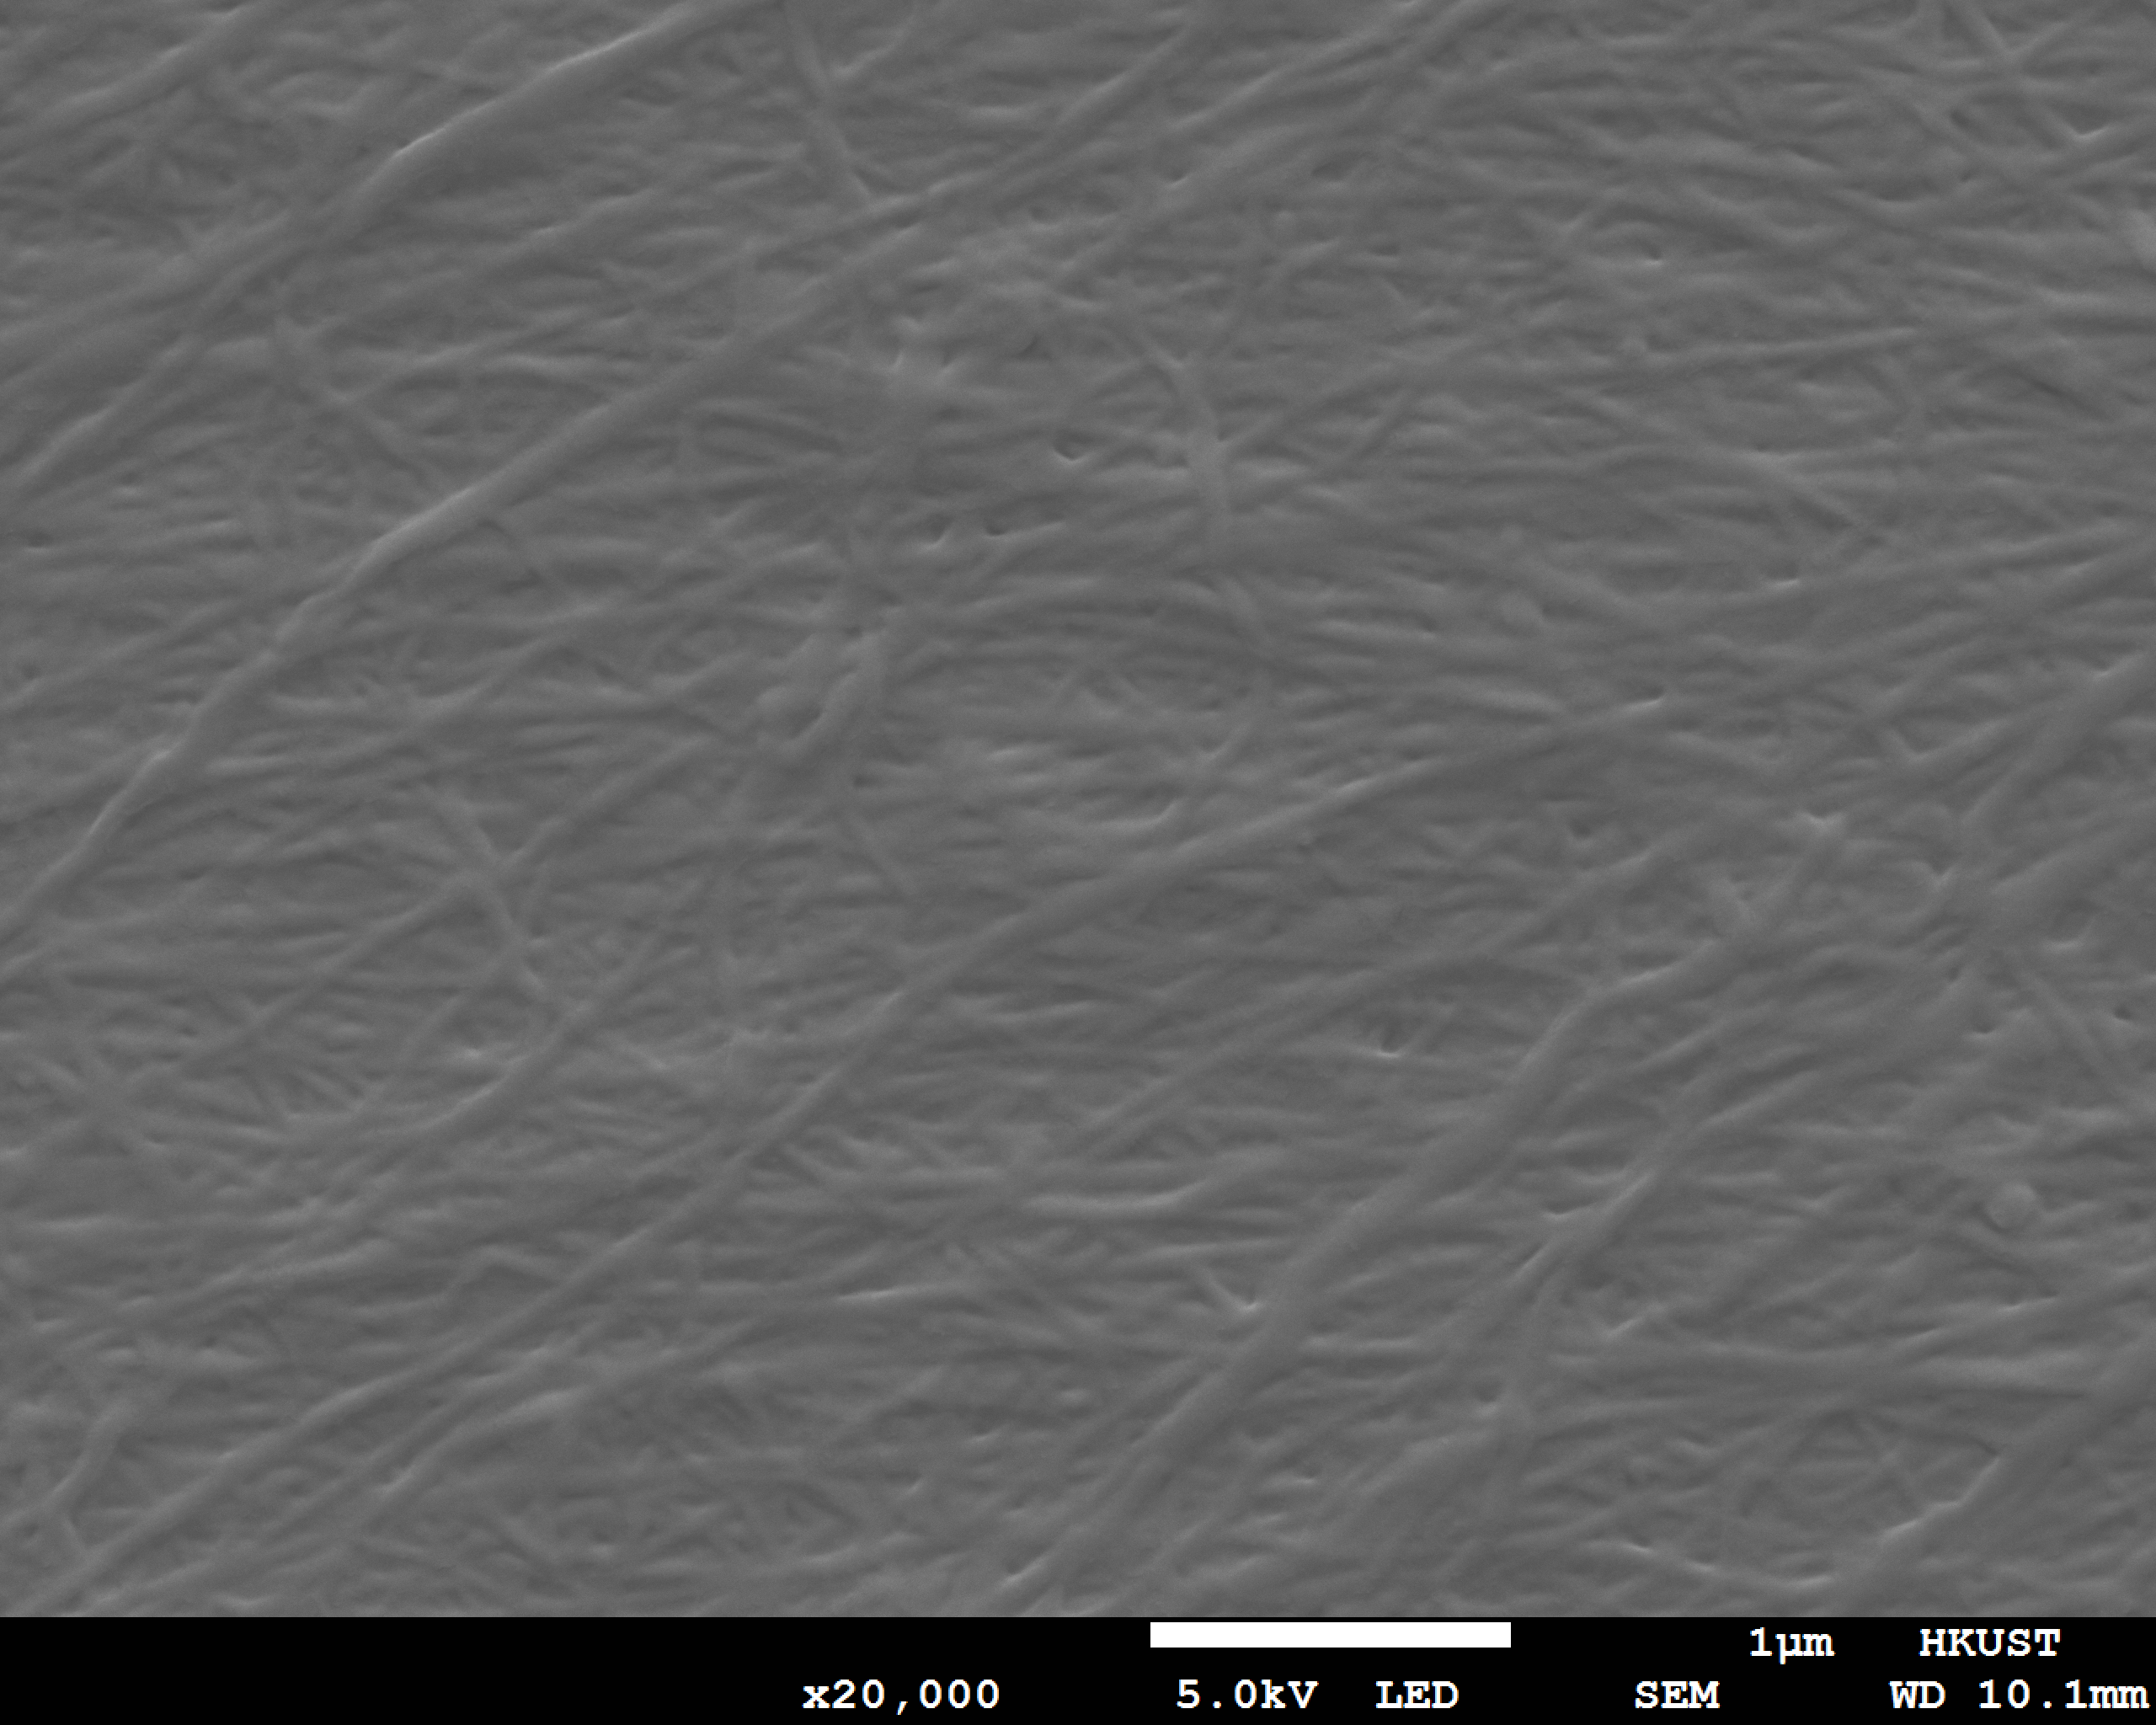
\includegraphics[width=0.23\textwidth]{images/sweated_p.png}
\includegraphics[width=0.23\textwidth]{images/control_C.png}
\includegraphics[width=0.23\textwidth]{images/sweated_C.png}
\caption{SEM micrographs. \textit{Upper left: Control Sensor-P. Upper right: Sweated Sensor-P. Bottom left: Control Sensor-C. Bottom right: Sweated Sensor-C}} \label{fig:sem}
\end{center}
\end{figure}

Silicon Dioxide (SiO$^2$) wafer is used as a placeholder for the samples; it results in a higher oxygen content in Table~\ref{tab:sem} than the expected 1:1 ratio from ZnO. The data obtained from EDS is then further calculated without Silica. Based on Table~\ref{tab:sem}, the sweat sensor is capable to sense biomarkers from sweat, shown by the presence of salt content (Na and Cl) in the sweated Sensor-C. 

\begin{table}[H]
\begin{center}
\caption{Mole distribution of components found in the control Sensor-C and the sweated Sensor-C using EDS} \label{tab:sem}
\includegraphics[width=0.48\textwidth]{images/asd.PNG}
\end{center}
\end{table}

\section{Discussion}
\subsection{Conformability}

The membrane thickness plays an important role to the conformability of the membrane. The Van der Waals force is the interacting force which holds the membrane and the skin together. Ethanol is used to remove the air bubbles between the skin and the membrane. The Van der Waals force is created when the ethanol, which replaces air gap between membrane and skin, dries out and builds laplace pressure. As the membrane gets thinner, its surface roughness also decreases, which leads to closer gap between the skin and the membrane. Then, a stronger Van der Waals force is generated between the two surfaces and able to support the membrane to have better resistant to any skin movement. The force can be calculated based on Equation~\ref{eq:van}, where P is pressure, C is a constant (10$^{-19}$ Joules), A is area and D is distance between two surfaces. 

The Van der Waals force (F) is inversely proportional with the distance (D) to the power of three. With the gap between 1 and 10 nm, shorter gap results in stronger Van der Waals force. Hence, with the membrane flexibility supported by the Van der Waals force, the nano-level thickness membrane adheres strongly on the skin surface. Thus, it can be concluded that with thickness of approximately 100-200 nm, the membrane can be fully conformed on the skin surface independently or without any help from external supports.

\begin{equation}
    F = \frac{P}{A} = \frac{C * A}{6 * \pi * D^3} 
    \label{eq:van}
\end{equation}

Bending modulus is also a crucial factor to ensure the membrane conformability. It is used to measure the resistance out of plane deformation. It was found that Bending Modulus of the membrane ranges from 5.2x10$^{-11}$ to 1.5x10$^{-12}$Pa.m$^3$. The smaller the bending modulus, the  Despite having thickness of nanometer scale, the bending modulus value of the UHMWPE membrane is still 2000 times higher than steel, which has a bending modulus value of 638 MPa~\cite{SheerStrength}. Calculating the skin bending modulus using the same formula, the result ranges from 9.4x10$^{-8}$ to 1.14x10$^{-7}$ Pa.m$^3$, which is higher than the bending modulus value of the membrane. This proves that the membrane has higher ability to deform compared to skin. Hence, the flexibility and elasticity of the membrane validates its capability to handle high bending force before it is torn or broken. 

\subsection{Breathability}

As mentioned in the literature review, human can produce up to 10-14 litre of sweat each day, whereas during moderate exercises, it can reach up to 2-4 litre per hour. Using the average surface area of male adult’s skin which is 1.8 m$^2$~\cite{BenderDict}, and Eq.~\ref{eq:pass_rate}, the human sweat rate is calculated to be about 6.43 $\pm$ 3.6 x 10$^{-8}$ m$^3$/(m$^2$.s) without exercise and 3.09 $\pm$ 3.06 x 10$^{-7}$ m$^3$/(m$^2$.s) during exercise.  

Comparing human sweat rate with the sensor breathability rate, it is found that the sweat sensor is 200-1000 times faster than the human perspiration rate. It proves that the membrane is capable to cope with the human perspiration and makes it breathable for the skin. Due to this breathability, the membrane application will not suffocate or make rash on skin.

\subsection{Raman}

It was proven that the sensor is able to detect the cortisol from sweat. However, the cortisol peak compared to the polyethylene peaks are not significantly high enough to be optimally analysed. Hence, zinc-oxide (ZnO) nanoparticles was introduced to Sensor-P to enhance the cortisol peak in Raman Spectrometry. 

ZnO has the ability to immobilize the sweat biomarkers, which in the case of cortisol is by binding to its hydroxyl group. The ZnO nanoparticles can react to both acids and alkalis to give free Zn$^{2+}$ ions, which can immediately bind with the sweat biomarkers such as hormone and glucose, forming Zn-biomolecule complex~\cite{PropertiesZnO}. Figure~\ref{fig:cortisol_raman} proves the ZnO nanoparticles ability to cause further Raman shifts from the O-H bond present in cortisol through higher cortisol intensity compared to the sample without the addition of ZnO. From the result, it is proven that the ZnO nanoparticles can immobilize the cortisol, increasing the collection of cortisol in sweat by the sensor and causing better detection and analysis of fatigue. 

\subsection{Biocompatibility}

In recent years, UHMWPE membrane has been implemented in many biomedical applications due to its properties, such as the wear and fatigue resistance, as well as the biocompatibility of the material. It has been widely used to reconstruct damaged body parts, including hip and knee joint replacements. In order to prove its biocompatibility, the cytotoxicity of UHMWPE was checked by incubating fibroblast (L929) with the polyethylene material in a culture medium. The result illustrated an identical growth of the cells as in a cultural plate, which indicates the biocompatibility of UHMWPE. If that particular material is safe enough to be a replacement of human body parts, then its usage on skin surface is definitely considered to be safe~\cite{UHMWPEBiocompatibility}. 

Zinc oxide which is introduced in Sensor-C has been used especially in biosensing application due to its high catalytic efficiency, strong adsorption ability, fast electron transfer kinetics, and biocompatibility. These properties of ZnO enable immobilization of biomolecules as ZnO particles can have high sensitivity and high affinity binding to organic materials, such as glucose and uric acid [19]. In addition, ZnO nanoparticles have been extensively used as one of the major building blocks of sunblock, sunscreen, and several cosmetics which is proven to be safe for usage on the skin~\cite{ZnO}. Therefore, it can be concluded that both UHMWPE and ZnO are biocompatible and thus safe to be used directly in contact with the skin

\subsection{Cost and Market Analysis}
\subsubsection{Sensor-P Cost}

The raw cost needed to fabricate a single Sensor-P is calculated by dividing the price of raw UHMWPE with the weight of a single sensor. The price of one kilogram of raw UHMWPE in the market equals to 40 US\$. A single piece of Sensor-P has the weight up to 10$^{-5}$ gram. Thus, the price of each unit equals to 4 x 10$^{-7}$ US\$.

\subsubsection{Sensor-C Cost}
Whereas the cost for Sensor-C is the cost needed to build a single Sensor-P added with ZnO nanoparticle - Ethanol solution price. In the calculation, the assumptions used are 
\begin{enumerate}
    \item Density of Ethanol used is 789 kg/m$^3$
    \item Density of ZnO nanoparticle is very small compared to Ethanol and is neglected.
    \item Solution of 1 wt\% ZnO
    \item Volume of solution used for big frame (10 units of sensor) is 200 microliter 
    \item Price of ZnO is 34.15 US\$ / 10 gram~\cite{Sigma38}
    \item Price of Ethanol is 1318.76 US\$ / 16 L~\cite{Sigma39}
\end{enumerate}

It is found to fabricate 10 pieces of Sensor-C, 1.594 x 10$^{-3}$ gram of ZnO is used, and 200 x 10$^{-6}$ L of ethanol is used. Then, based on Equation~\ref{eq:price}, the price of a single piece of Sensor-C is 2.19 x 10$^{-3}$ US\$

\begin{equation}
    Sensor-C = Sensor-P + \frac{Price_{ZnO} + Price_{Ethanol}}{piece} 
    \label{eq:price}
\end{equation}

Considering the cost of a finger pricker which is up to 1 US\$~\cite{Blood}, with the same amount of money, up to 450 Sensor-C can be produced. This tremendous adding value to the raw material can bring Sensor-C to compete with other existing sport sensors in the market.

\subsection{Limitation}

Although the sensor is already proven to successfully able to pick up the cortisol, there are still some factors needed to be addressed to accurately measure the fatigue level. The current practice of analyzing the cortisol level is by implementing Raman Spectrometry, which illustrates that laboratory work is still required at this stage. Moreover, the experiment to test membrane capability to detect cortisol from human blood for comparison to the existing sweat detection has not been done. Thus, more experiment and data analysis on measuring the cortisol concentration that can be picked up by the membrane from human blood is still necessary to compare which one is the better source of cortisol collection. The abilities of the device to perform real time analysis and detect the cortisol limit per individual are also currently not available since the film has not been integrated with electronic sensor. 

\subsection{Future Work}
\subsubsection{Cortisol Quantification}

Integration with the molecular specific sensor or using a device such as portable Raman Spectrometry can also make cortisol quantification possible to increase the level of sensor’s accuracy. Due to its molecular-specific property, Raman Spectrometry enables the measurement of cortisol concentration excreted by the body through sweat collection. The amount of cortisol can be normalized with the amount of sodium chloride (salt) secreted by the body to better analyse the level of tiredness during the exercise. The salt concentration was obtained from the EDS data from Table~\ref{tab:sem}. The salt is used as the reference state because unlike water and small organic materials, it cannot evaporate from the sweat and hence the ratio of cortisol to salt will not fluctuate and high accuracy of the analysis can be obtained. 

\subsubsection{Sensor Integration for Real Time Analysis}

Further improvements of the sensor can be made by integrating the nanofilm with a sensor for real time analysis. Using the sensor to detect body temperature and cortisol level, the device can assist athletes to check their fatigue level anytime and anywhere. A future collaboration with HKSI is possible to further improve the fatigue detection for Hong Kong professional athletes. The current practice of cortisol level analysis in HKSI is measuring it before practices in order to check the athletes’ preliminary condition pre-exercise. Various reasons such as stress, nervousness and sickness can diminish physical condition of athletes. To minimize the risk of getting injured, the workout portion has to be adjusted according to the results acquired from fatigue tests. Having said that, just because of not having a perfect condition does not leave them out of their daily dose of workouts. There is no such method which is able to tell the athletes when they have actually reached their maximum limit and act as a strong indicator for the coach to halt the workout. Here is where the device comes as its complementary method. As our sensor is applied during the exercise, our membrane can immediately signal the users as soon as their cortisol level has already gone beyond acceptable ranges. 

\subsubsection{Personalised Device}

Realistically, each athlete has different physical ability which cannot be generalized by one specific ranges. That is why HKSI coaching staff has had a complete database of their athletes’ physical ability. They measured the cortisol and testosterone level under a perfect fit condition of the athletes and made it as their baseline level. The deviation from the baseline level is then used as the indicator of fatigue and it will be a far more accurate analysis since it is compared to the athlete’s own normal level. To accommodate that level of accuracy for the users, our membrane needs to be further integrated with big data technology. By that, we can store user’s physical database and signals its deviation when the cortisol exceeds their normal ranges.

\section{Conclusion}

This project has successfully improved athletes coaching system through preventing the overtrained cases and optimizing their physical performance. By using UHMWPE sweat sensing device, it is discovered that the sensor is capable of detecting cortisol - a hormone secreted by adrenal gland which is used as a more accurate indicator for sports fatigue detection instead of lactic acid and heart beat rate. The existing practise, particularly used in Hong Kong Sports Institute (HKSI), measures cortisol level where invasive blood testing is compulsory to be performed both before and after training sessions; this method is found to be very inconvenient for the athletes. Yet, the state-of-the-art non-invasive sweat sensors capable of sensing cortisol and monitoring fatigue~\cite{SkinSystems, UHMWPEMembrane, LabOnSkin} are both too bulky and non-breathable which interferes the sports activities. The nano-level thickness of the proposed device enables the full conformability to human skin and its properties mentioned before is the first of its kind worldwide which can improve athlete’s training programs.

The sweat sensing device can be further developed to provide a real-time analysis through the integration with electronic sensors which can notify users as soon as they exceed the normal benchmark. Furthermore, a more accurate measurement can be further achieved by using Big Data Technology which can store each user’s data and make it a more personalized device. Through these developments, the UHMWPE can definitely be a unique health monitoring device which revolutionizes the healthcare industry. 


\appendices
\section*{Acknowledgment}

We would like to acknowledge the help and guidance from Mr. Jin Li, Dr. Runlai Li from Prof. Ping  Gao’s  group, as well as our supervisor Prof. Ping Gao  regarding  the  sensor  material  preparation  and  several characterizations. The project would not be able to progress without their help. We also want to thank other parties that have been involved by helping us either directly or indirectly during the process

% Can use something like this to put references on a page
% by themselves when using endfloat and the captionsoff option.
\ifCLASSOPTIONcaptionsoff
  \newpage
\fi

\bibliographystyle{IEEEtran}
\bibliography{IEEEabrv,citation}

\end{document}